\documentclass[titlepage]{article}
\usepackage[a4paper, total={6in, 8in}]{geometry}

\usepackage{preamble}

\title{
    \textbf{COMPARISON OF \\
    HEURISTIC ALGORITHMS \\
    FOR KP01} \\[0.5cm]
    \rule{12cm}{0.3mm} \\[0.5cm] 
    \small \scshape{A comparison of heuristic algorithms for solving the 0-1 Knapsack Problem} \\[0.4cm]
    \rule{12cm}{0.3mm}
    \vskip -0.3cm
}

\author{
    \small \scshape{Raunak Redkar} \\ 
    \small \scshape{Supervisors: Per-Olof Freerks and Felicia Dinnetz} \\
    \scriptsize \scshape{Kungsholmens Gymnasium}
}

\begin{document}

\onehalfspacing

\maketitle

\newpage
\tableofcontents
\listofalgorithms
\newpage
\pagenumbering{arabic}

\section{Introduction}

\subsection{Background}

\renewcommand{\familydefault}{Computer Modern}
There are many situations in every day life, where a person wonders whether he is doing something efficiently. Unforunately, the human brain is not always capable of coming up with an optimal approach when the problem has a lot of factors at play. It is here when a system is used, and the true power of computing can be recognised. 

To solve such problems, a computer is provided all the information, from which it will produce an optimal answer. For the system to process all the information, certain instructions must be written into the system so that it knows how to handle the information. This set of instructions is called an algorithm. The system or computer uses algorithms to take in information (the input), and produce an answer - an output. The efficiency (in all aspects) of the algorithm is dependant on the instructions which make up it. There are many algorithms which have been designed to solve many problems. For problems in computer science, more than one algorithm is usually proposed and used. Optimization problems are where this is frequently the case. 

In the fields of computer science and mathematics, optimization problems are problems of finding the best solution, from a range of many feasible solutions. They are usually categorized into 2 categories: discrete optimizations and continuous optimizations, depending on whether the variables are discrete or continuous respectively. Combinatorial optimization problems are a subset of optimization problems that fall into the discrete. Combinatorial optimization involves searching for a maxima or minima for an objective function whose search space domain is a discrete but (usually large) space.

Typical combinatorial optimization problems are not limited to but include:
\begin{itemize}
    \item \textcolor{blue}{General Knapsack Problem} - Given a set of items, each with weight and profit value and a knapsack capacity, what is the best way to choose the items while respecting the knapsack capacity?
    \item \textcolor{blue}{Traveling Salesman Problem}- Given a list of cities, what is the shortest possible path that visits each city exactly once and returns to the origin?
    \item \textcolor{blue}{Set Cover} - Given a set of elements $\{1, 2, ..., n\}$ , what is the and a collection of $m$ sets whose union equals the universe, what is the smallest sub-collection of sets whose union is the universe?
\end{itemize}

Combinatorial optimization problems show up in an array of different fields. The Knapsack Problem in particular has many variants which include the 0-1 knapsack problem, the bounded and unbounded knapsack problems, the multidimensional knapsack problem, the discounted knapsack problem, etc. The 0-1 Knapsack Problem is the simplest form of the knapsack problem and thus has also been the main focus in the research community. It appears in real-world decision-making processes in a variety of fields. Some examples include: 

Many of combinatorial optimization problems including the 0-1 Knapsack problem currently do not have deterministic algorithms which are considered fast enough for them to be used on a large-scale basis. Consequently, the research focus has been on approaches that do not necessarily guarantee the best solution but win over deterministic approaches when it comes to time. 

\subsubsection*{Problem statement}
In the 0-1 Knapsack Problem, there $n$ items and a maximum weight capacity $W$. Each item has a profit value $p_i$ and a weight value $w_i$. Find the optimal selection of items which maximizes the profit value while respecting the max weight value. The problem can be mathematically represented as so:

\vskip -0.5cm

\begin{gather}
    \text{Maximize}\;\; f(\Vec{x}) = \sum_{i = 1}^{n} p_i x_i \\
    \text{subject to} \sum_{i = 1}^{n} w_i x_i <= W \\
    x \in \{0, 1\}
\end{gather}

The rest of this paper will follow the shorthand "KP01" for the 0-1 Knapsack Problem. 

\subsection{Aim}
The aim of this paper is to compare algorithms in order to investigate the strength of commonly used techniques in for solving optimization problems.

\subsection{Research Question}
How do the global-best harmony search algorithm and the binary harmonic multi-scale algorithms perform when implemented for solving KP01?

\section{Theory}
\subsection{Computational Complexity}
In computer science, computational complexity is the measure of how expensive it is to the run an algorithm; the amount of resources required to run the algorithm. The 2 resources are time and memory, notated time complexity and space complexity. As the memory complexity is dependent on the time complexity, the time complexity is the limiting factor for the efficiency of an algorithm and is usually the one focused on. Computable problems can be factorial, exponential, polynomial, logarithmic, etc.

\subsubsection*{Big O notation}
The time complexity of an algorithm is a function of the size of the input of that algorithm. For example, if $n$ numbers $a_1, a_2, a_3, ..., a_n$ are given, and an algorithm checks the existence of an certain element in those numbers, by checking all n elements, then the time complexity is some constant times $n$ - the size of the input. Computer scientists would denote this using Big O notation as $\mathcal{O}(n)$. Big O notation is a system developed by mathematicians and computer scientists to describe an function/algorithm's asymptotic limiting factor.

Computer scientists usually categories the time complexity of an algorithm into polynomial time complexities and non polynomial time complexities. This is because non-polynomial functions like factorial and exponential functions tend to grow quicker than polynomial functions and thus are usually considered nonviable for large data. 

\vskip 1cm

% time complexities graph
\begin{center}
    \begin{tikzpicture}
      \begin{axis}[
          grid = major,
          clip = true,
          ticks = none,
          width=1\textwidth,
          height=0.8\textwidth,
          every axis plot/.append style={very thick},
          axis line style = ultra thick,
          clip mode=individual,
          restrict y to domain=0:10,
          restrict x to domain=0:10,
          axis x line = left,
          axis y line = left,
          domain = 0.00:10,
          xmin = 0,
          xmax = 11,
          ymin = 0,
          ymax = 11,
          xlabel = n,
          ylabel = Computer Operations,
          xlabel style = {at={(axis description cs:0.5,-0.1)},anchor=south},
          ylabel style = {at={(axis description cs:-0.08,0.5)},anchor=north},
          label style = {font=\LARGE\bf},
          ]
          \addplot [
            samples=100,
            color=red, 
          ] gnuplot{gamma(x+1)*3^x} node[above,pos=1,style={font=\Large}]{$\mathcal{O}(n!\cdot3^{n})$};
          \addplot [
            samples=100, 
            color=orange,
          ]
          {2^x}node[above,pos=1,style={font=\Large}]{$\mathcal{O}(2^{x})$};
          \addplot [
            samples=100, 
            color=green,
          ]
          {x}node[above,pos=1,style={font=\Large}]{$\mathcal{O}(n)$};
          \addplot [
            samples=100, 
            color=blue,
          ]
          {log2 x}node[above,pos=1,style={font=\Large}]{$\mathcal{O}(\log{}n)$};
          \addplot [
            samples=100,
            color=violet,
          ]
          {2*sqrt x}node[above,pos=1,style={font=\Large}]{$\mathcal{O}(2\sqrt{n})$};
          \addplot [
          samples=100, 
          color=red,
          ]
          {1}node[above,pos=1,style={font=\Large}]{$\mathcal{O}(1)$};  
            
      \end{axis}
    \end{tikzpicture}
\end{center}

\paragraph{\textbf Solving the 0-1 Knapsack Problem} \mbox{}\

There are 2 main approaches to solving KP01: An exact solution using deterministic algorithms, and probabilistic approaches involving heuristic algorithms. A small-scale KP01 can be solved with deterministic approaches, but for high-scale situations it is not realistic to get optimal solutions with exact approaches \cite{QWPA} as the KP01 problem is NP-complete \ref{some website}.

\subsection*{Deterministic algorithms}
Dynamic programming is a general technique for solving optimization problems. If a problem has optimal substructure and over-lapping subproblems, then dynamic programming is applicable. In computer science 
a problem has \emph{optimal substructure} if an optimal solution for a problems can be constructed from optimal solutions of its sub-problems, and \emph{over-lapping subproblems} is when a problem can be decomposed into sub-problems which are reused. Dynamic programming breaks down a complicate problem into smaller sub-problems in a recursive manner, while also using some memory to save the solutions of the sub-problems (usually in tabular form). This way, when we need to get a solution for a sub-problem again, we can just use our previously calculated value. 

KP01 is solved using dynamic programming using a table based computation:

%dp
\begin{breakablealgorithm}
\caption{Solving 0-1 Knapsack with Dynamic Programming}\label{dp}
    \begin{algorithmic}[1]
        \For {$i = 0 \text{ to } noItems $} \Comment{\textcolor{blue}{If no items, then profit = 0}}
            \State $Table[i][0] \gets 0 $ 
        \EndFor
        \For {$k = 0 \text{ to } maxCapacity $} \Comment{\textcolor{blue}{If no capacity, then profit = 0}}
            \State $Table[0][k] \gets 0 $
        \EndFor
        \For {$i = 0 \text{ to } noItems$}
            \For {$k = 0 \text{ to } maxCapacity $}
                \State $Table[i][k] \gets Table[i-1][k]$  
                \If {$k-weights[i] >= 0$} 
                    \State $Table[i][k] \gets max(Table[i-1][k-weights[i]] + profits[i], Table[i][k]) $
                \EndIf
            \EndFor
        \EndFor
        \State $\textbf{Print } Table[noItems][maxCapacity] $
    \end{algorithmic}
\end{breakablealgorithm}

\vskip 0.5cm

This implementation of dynamic programming method has a time complexity of $\mathcal{O}(N\cdot W)$, where N is the number of items, and W is max capacity. The dynamic programming algorithm does not end until the entire table is built. This proves to be inefficient very quickly as the maximum capacity and the number of items in the knapsack increases. So with the increase in the scale, the feasibility of dynamic programming decreases which has incentivized research in the subfield of heuristic algorithms.

\subsection*{Heuristic algorithms}
When deterministic algorithms prove to be too slow for practical applications, heuristic algorithms are chosen for their (usually) near optimal outputs and their speed. Heuristic algorithms should not be confused with approximation algorithms. Approximation algorithms guarantee a maximum margin of error; a constant factor off of the optimal. On the other hand, a heuristic algorithm does not guarantee anything, so it can perform better or worse than an approximation algorithm. 

Heuristic algorithms for combinatorial optimization are usually designed in a specific way \ref{some website}:
\begin{enumerate}
    \item Create a potential solution which is current best.
    \item Generate new solution. (usually in polynomial time) 
    \item If new solution better than current best, swap out the best with the newly generated. 
    \item If satisfied, output best solution, else continue.
\end{enumerate}

Both the Discrete Global-Best Harmony Search (DGHS), and Binary Multi-Scale Quantum Harmonic Oscillator (BMQHOA) have a similar framework.

\subsubsection{Discrete Global-Best Harmony Search Algorithm}
The Harmony Search algorithm (HS) was developed in 2001 \cite{geem01} based on the improvisation of music players \textcolor{red}{EXPAND}. This algorithm was made for continuous search spaces and thus cannot be used for discrete search spaces in combinatorial optimization problems. The Discrete Global-Best harmony search was proposed by Wan-li Xiang et al. \cite{DGHS-article} \textcolor{red}{EXPAND} to overcome this. The DGHS for KP01 also has a repair-operator and a greedy selection mechanism. A harmony in this algorithm refers to a candidate solution, or a certain selection of items to be put in the knapsack. 

It consists of 4 main parts:
\begin{enumerate}
    \item Create a harmony memory HM - a fixed size (HMS) of randomly generated harmonies. Initialize parameters harmony memory consider rate (HMCR), and pitch adjusting rate (PAR), and calculate profit-density vector for usage in the repair-operator.
    \item Create a new harmony using the current HM \ref{harmonyGen}.
    \item If generated harmony is better than the best in the harmony, replace it. If not, check if it is better than then worst harmony, and replace it if so. 
    \item If maximum number of iterations has been met, output the best sum profit value found so far.
\end{enumerate}

\vskip 0.5cm
%DGHS
\begin{breakablealgorithm}
\caption{The DGHS algorithm}\label{DGHS}
    \begin{algorithmic}[1]
        \State Set the harmony memory size $HMS$, the number of iterations $ITERATIONS$, and the minimum and maximum values of parameters $PAR$ and $HMCR$.
        \State Initialize the HM through a randomized process, and use \ref{harmonyRepair} to the generated harmonies. Calculate the totalProfit and totalWeight values for each harmony in HM.
        \State $iterator \gets 1$
        \While {$iterator <= ITERATIONS$}
            \State Record indices of the best and the worst harmonies in HM.
            \State Calculate parameters HMCR and PAR for the current iteration.
            \State Perform Algorithm \ref{harmonyGen} to produce a new harmony $\Vec{x}_{new}$
            \State Perform Algorithm \ref{harmonyRepair} to repair the new harmony $\Vec{x}_{new}$
            \If {$\Vec{x}_{new} \text{ is better than or equal to } \Vec{x}_{best}$}
                \State Replace $\Vec{x}_{best} \text{ with } \Vec{x}_{new}$
            \ElsIf {$\Vec{x}_{new} \text{ is better than or equal to } \Vec{x}_{worst}$}
                \State Replace $\Vec{x}_{worst} \text{ with } \Vec{x}_{new}$
            \EndIf
            \State $iterator \gets iterator+1$
        \EndWhile
        \State Output profit of best harmony
    \end{algorithmic}
\end{breakablealgorithm}
\vskip 0.5cm

The parameters HMCR and PAR are used when generating new harmonies. They determine the likelihood of heading toward the current best harmony, and the likelihood of randomly flipping a decision variable. The idea is that current best harmony should have an influence on the generation of a new harmony, and that a decision variable (whether or not an item is put in the knapsack) should be flipped to allow for diversity in the HM, making it easier to overcome local maxima. These parameters are determined in terms of the current iteration like so:

\begin{equation}
    HMCR(t) = HMCR_{max} - \frac{HMCR_{max}-HMCR_{min}}{ITERATIONS} t
\end{equation}
\begin{equation}
    PAR(t) = PAR_{max} - \frac{PAR_{max}-PAR_{min}}{ITERATIONS} t
\end{equation}

The dynamic updating of the parameters is designed in this way to let larger values of HMCR help accelerate the convergence of the harmonies early on with the the help of the best individual harmony, while smaller values of HMCR can help you overcome local maxima \cite{DGHS-article}. Similarly, larger values of PAR in the beginning allow for increases in diversity through mutations (item decision bit flips), when there is time to "explore" different variants, smaller values allow convergence at the end of the search. 

With these parameters one generates a new harmony:

%harmonyGen
\begin{breakablealgorithm}
\caption{Generating a new harmony during iterative part (part 2)}\label{harmonyGen}
    \begin{algorithmic}[1]
        \For {$i = 1 \text{ to } noItems$}
            \If {$rand(0, 1) <= HMCR(t)$}
                \State $newHarmony[i] \gets bestHarmony[i]$ 
            \Else
                \State Generate a random integer number $a \in \{1, 2, ... HMS\}, a \neq best$
                \State $newHarmony[i] \gets Harmony_{a}[i]$ 
                \If {$rand(0, 1) <= PAR(t)$}
                    \State $newHarmony[i] = |newHarmony[i]-1|$ \Comment{\textcolor{blue}{Flipping i'th item - mutation}}
                \EndIf
            \EndIf
        \EndFor
    \end{algorithmic}
\end{breakablealgorithm}
\vskip 0.5cm


Any time a harmony is generated, during Part 1 or Part 2, it is "repaired" in case the selection of items exceeds the capacity of the knapsack. The new generated harmony is also repaired if it can fit more items, without exceeding the capacity of the knapsack. The repair-operator consists of 2 phases:
\begin{enumerate}
    \item Drop phase - repairing a harmony if it violates the constraint
    \item Add phase - adding a items into the knapsack if the total weight is less than the capacity
\end{enumerate}

The add phase is always done after the drop phase, as a harmony previously infeasible becomes feasible after the drop phase, but its total weight may be less than the capacity of the knapsack. Here is the pseudocode for the repair-operator:

\vskip 0.5cm
%harmonyRepair
\begin{breakablealgorithm}
\caption{Repair-operator for DGHS}\label{harmonyRepair}
    \begin{algorithmic}[1]
        \If {$totalWeight > maxWeight$}
            \For {$i = 1 \text{ to } N$} \Comment{\textcolor{blue}{DROP phase}}
                \State $\lambda_{i} = \frac{profit_{i}}{weight_{i}}$
            \EndFor
            \State Sort items in increasing order of $\lambda_{i}$, and let $ind_{i}$ denote the original index of each $\lambda_{i}$
            \For {$i = 1 \text{ to } noItems $} 
            \State Remove the ones with the least profit-density values greedily
                \If {$\lambda_{i} == 0$}
                    \State \textbf{Continue}
                \EndIf
                \State $newHarmony[ind_{i}] = 0$ \Comment{\textcolor{blue}{Unload the item}}
                \State $totalWeight \gets totalWeight - weight[ind_{i}]$
                \State $totalProfit \gets totalProfit - profit[ind_{i}]$
                \If {$totalWeight <= maxWeight$}
                    \State \textbf{Break} \Comment{\textcolor{blue}{Terminate DROP phase}}
                \EndIf
            \EndFor
        \EndIf
        \If {$totalWeight < maxWeight$}
            \For {$i = 1 \text{ to } N$} \Comment{\textcolor{blue}{ADD phase}}
                \State $\lambda_{i} = \frac{profit_{i}}{weight_{i}}$
            \EndFor
            \State Sort items in increasing order of $\lambda_{i}$, and let $ind_{i}$ denote the original index of each $\lambda_{i}$
            \For {$i = 1 \text{ to } noItems $} 
                \State Add the ones with the greatest profit-density if possible 
                \If {$newHarmony[ind_{i}] == 0$}
                    \If {$totalWeight + weight[ind_{i}] <= maxWeight$}
                        \State $newHarmony[ind_{i}] = 1$
                        \State $totalWeight \gets totalWeight + weight[ind_{i}]$
                        \State $totalProfit \gets totalProfit + profit[ind_{i}]$
                    \EndIf
                \EndIf
            \EndFor
        \EndIf
    \end{algorithmic}
\end{breakablealgorithm}

\vskip 1cm
\subsubsection{Binary Multi-Scale Quantum Harmonic Oscillator Algorithm}

The Multi-Scale Quantum Harmonic Oscillator Algorithm (MQHOA) is called such as it follows a model of a solving a particle's ground state wave function under the harmonic oscillator potential well \cite{BMQHOA-article} . In MQHOA, candidate solutions are generated by sampling points in a Gaussian distribution within a certain distance of something. The Binary Multi-Scale Quantum Harmonic Oscillator Algorithm (BMQHOA) discretizes this by defining the number of bits between solutions (item decision variable ) as the distance between solutions, so it becomes a discrete search space. Similar to the DGHS algorithm, a repair-operator is added fix solutions which violate the capacity constraint. 

The BMQHOA algorithm consists of 4 parts:
\begin{enumerate}
    \item Random binary vector generation -> repair
    \item Generating a solutions by flipping $m$ items, mutating, and repairing
    \item Reducing the standard deviation value for the normal distribution from which $m$ is determined every iteration.
    \item If termination constraint is satisfied, output best totalProfit value, else return to Step 2.
\end{enumerate}

%BMQHOA
\begin{breakablealgorithm}
\caption{The BMQHOA algorithm with solution generation}\label{BMQHOA}
    \begin{algorithmic}[1]
        \State Set the number of iterations $ITERATIONS$ and the number of binary vectors (solutions) - BINVEC in memory.
        \State Randomly generate the binary vectors and use Algorithm \ref{harmonicRepair} to repair the vectors. 
        \While {$iterator <= ITERATIONS$}
            \State Update $\sigma_{s}$
            \State $found \gets FALSE$
            \While {$found == FALSE$}
                \State Try to generate a solution
                \State Let $solutions_{new}$ be the new generated vector 
                \State $solutions_{new} \gets solutions_{best}$
                \State Generate the number of flipped bits $m ~ N(0, \sigma_{s})$
                \State Treat $solutions_{new}$ as a circular array
                \State Randomly select a position in $solutions_{new}$ and flip the next $m$ items.
                \State Mutate a random bit towards current best solution (flip an item)
                \State $solutions_{new}[rand] \gets solutions_{best}[rand]$
                \State Repair newly generated solution
                \If {$totalProfit >= totalProfit_{worst}$}
                    \State Replace worst solution with newly generated solution
                    \State $solutions_{worst} \gets solutions_{new}$
                    \State $found = TRUE$
                \EndIf
            \EndWhile
        \EndWhile
    \end{algorithmic}
\end{breakablealgorithm}
\vskip 0.5cm

After generating a new solution, $m$ items are flipped in the hope of increasing diversity in the solutions and increasing the likelihood of finding the optimal solution. They are generated randomly with a normal probability distribution around \textbf{0}, with a mean of $0$ and a variable std deviation. The Std. Deviation decreases with each new-solution-generation iteration so as to increase diversity in the beginning of the search, while reducing the likelihood of corrupting a binary vector closer to the end of the search when close to optimal solutions have (hopefully) been found. Initially the value of the standard deviation is set to $noItems/3$, so that there is a $\sim 99.7\%$ chance that the generated number of flipped items $m$ are in the range $[0-3\sigma_{s}, 0+3\sigma_{s}] \approx [-noItems, noItems]$:
$$STDEV_{max} = noItems/3$$
$$\sigma_{s} = 1-\frac{t}{ITERATIONS} STDEV_{max}$$


The normal distribution probability density function generator is implemented with the C++ Standard Library class normal\_distribution. An item's decision value is also made to match the corresponding decision in the best solution, which gives a slow mutation towards the current best solution allowing for diversity while still allowing the best solution to influence the process. Allowing multiple bits to mutate toward current best, this can lead to a premature local maximum, nullifying the rest of the search \cite{BMQHOA-article} . 

The repair-operator of the BMQHOA algorithm has 3 phases:
\begin{enumerate}
    \item Density-first stage: The already selected items are sorted based on their profit to weight ratio in non-increasing order and then greedily selected while respecting the weight constraint. 
    \item Minimum-weight-first stage: Out of the items that weren't selected in the first stage are sorted based on their weight values in non-decreasing order, then greedily selected while respecting the weight constraint.   
\end{enumerate}

$Q_{1}[1, 2,...,n]$ is the index for the items in the density ratio array in the original vector. $Q_{2}[1, 2,..., n]$ is index of the items in the minimum weight sorted array in the original vector.

\begin{breakablealgorithm}
\caption{Repair-Operator for BMQHOA}\label{harmonicRepair}
    \begin{algorithmic}
        \State Let $x$ be the current array/vector.
        \State $totalWeight = 0, temp = 0, i = 0, b = 0$
        \State Stage 1: Density first stage
        \While {$temp < maxWeight$}
            \State $totalWeight = temp$
            \State $i += 1$
            \State $temp = temp + weight[Q_{1}[i]]$
        \EndWhile
        \For {$j = i \text{ to } n$}
            \State $x[Q_{1}[j]] = 0$
            \State $totalWeight += x[Q_{1}[j]]$
        \EndFor
        \State Stage 2: Minimum weight first stage
        \While {$totalWeight < C$}
            \State $b += 1$
            \If {$totalWeight + weight[Q_{2}[b]] <= C$} 
                    \State $x[Q_{2}[b]] = 1$
                \State $totalWeight += weight[Q_{2}[b]]$
            \EndIf
        \EndWhile
    \end{algorithmic}
\end{breakablealgorithm}

\newpage

\section{Not finished - Methodology}

Testdata is made up of different testcases, each of which is an input on which every algorithm is run.

\subsection{Generating testdata}

3 testgroups of 5 testcases were made using a random number generator, where a random number was generated using the Mersenne Prime Twister (mt19937). A computer cannot generate a truly random number. A pseudorandom number is what is generated, which is a number which appears to be statistically random, but has been generated using a deterministic process. The 3 groups had item counts of 100, 1000, and 10000. The number of solutions in memory (for the heuristic algorithms) was put in the input file which was kept constant, 20, in all testcases and algorithms for this report. In the random number generated testcases, the number of items $n$ was chosen to either be 100, 1000 or 10000. The profit and weight values were then randomly generated in a range of $ [1, noItems] $ while a sum-of-weights variable \emph{sum} was kept. The max weight was then randomly generated in a range of $[\frac{\text{sum}}{100} , \frac{\text{sum}}{10}]$, so that the knapsack wouldn't be able to hold all the items. To avoid any overflow errors, all generated numbers (and the sum of the profit/weight values) were kept below the max value of an \emph{int} which is $2^{31}-1$ in many programming languages.  Then $n$, $W$ (maxWeight), and each item (profit and weight values) was put in an input file. To make a fair comparison the number of $ITERATIONS$ (how many times a candidate solution is generated) was set to 100 for both algorithms. 

3 groups of five testcases were taken from a database \ref{some website}. These 3 "testgroups" are mentioned/used several times in the literature. The 3 testgroups are uncorrelated, weakly correlated, and strongly correlated; the correlation being between the items' profit and weight values. The number of solutions in memory (20) was added to each of these testcases taken from \ref{some website}. 

These input files were then saved for later testing of the algorithms. 

Each testcase was then run on each algorithm and saved in a spreadsheet producing a csv table, refer to appendix.

\newpage

\section{Not finished - Results}

\subsection{Raw Data}
Refer to the appendix for the \hyperlink{random100}{raw data} for the algorithms running on the six testgroups: 100, 1000, 10k randomized numbers respectively and 3 differently correlated datasets. 
% \href{https://github.com/raunakCode/diploma-project/blob/main/testing/algorithms%20results.csv}{\textcolor{purple}{Link to results}}

\subsection{Processed Data}
The mean and standard deviations for each group can be viewed in the following corresponding tables and graphs:

\begin{table}[h!]\centering
    \caption{Mean and StDev. of 100 Randomized items} \label{100-mean}
    \begin{tabu}{|c|[1pt]c|c|c|c|c|c|}
        \tabucline[1pt]{1-6} 
        Testcase & 1 & 2 & 3 & 4 & 5 \\ [-1pt] \tabucline[1pt]{1-6} 
        DGHS Mean &4160.33 &2561 &5288 &3535 &1747 \\ \hline
        DGHS StDev. &3.50 &0 &19.66 &0 &0 \\ \hline
        Mean Percent deviation from optimal &0.21 &0.00 &0.40 &0.00 &0.00 \\ [-1pt] \tabucline[1pt]{1-6}
        BMQHOA Mean &3926.83 &2561 &4879 &3360.66 &1711.5 \\ \hline
        BMQHOA StDev. &40.27 &0 &46.18 &68.96 &25.71 \\ \hline
        Mean Percent deviation from optimal &5.80&0 &8.09&4.93&2.03\\ [-1pt] \tabucline[1pt]{1-6}
    \end{tabu}

    \vspace{1cm}
    
    \caption{Mean and StDev. of 1000 Randomized items} \label{1000-mean}
    \begin{tabu}{|c|[1pt]c|c|c|c|c|c|}
        \tabucline[1pt]{1-6} 
        Testcase & 1 & 2 & 3 & 4 & 5 \\ [-1pt] \tabucline[1pt]{1-6} 
        DGHS Mean &156083.83 &118603.83 &144070 &109734.33 &126366.16 \\ \hline
        DGHS StDev. &830.04 &1904.69 &1343.77 &1037.03 &1236.73 \\ \hline
        Mean Percent deviation from optimal &13.71&11.76&14.12&10.77&13.27\\ [-1pt] \tabucline[1pt]{1-6}
        BMQHOA Mean &145086.5 &109876.33 &136622.66 &101951.33 &118291.16 \\ \hline
        BMQHOA StDev. &1035.45 &1540.63 &2042.95 &1271.88 &799.78 \\ \hline
        Mean Percent deviation from optimal &19.79&18.25&18.56&17.10&18.82\\ [-1pt] \tabucline[1pt]{1-6}
    \end{tabu}

    \vspace{1cm}
    
    \caption{Mean and StDev. of 10k Randomized items} \label{10k-mean}
    \begin{tabu}{|c|[1pt]c|c|c|c|c|c|}
        \tabucline[1pt]{1-6} 
        Testcase & 1 & 2 & 3 & 4 & 5 \\ [-1pt] \tabucline[1pt]{1-6} 
        DGHS Mean &7681910.33 &10567302 &8014906 &9347061.66&9583139.16\\ \hline
        DGHS StDev. &51555.39&23956.31&39449.15&56967.66&55816.60\\ \hline 
        Mean Percent deviation from optimal &22.61&23.11&22.07&23.10&23.00\\[-1pt] \tabucline[1pt]{1-6}
        BMQHOA Mean &7438487.16&10276681.83&7774520.83&9075476 &9330322.16\\ \hline
        BMQHOA StDev. &29887.17&50507.35&34559.10&53168.02&46301.35\\ \hline 
        Mean Percent deviation from optimal &25.07&25.22&24.41&25.33&25.03\\[-1pt] \tabucline[1pt]{1-6}
    \end{tabu}
\end{table}

   % \vspace{1cm}
\begin{table}[h!]
    \centering
    \caption{Mean and StDev. of Uncorrelated Dataset} \label{uncorrelated-mean}
    \begin{tabu}{|c|[1pt]c|c|c|c|c|c|}
        \tabucline[1pt]{1-6} 
        Testcase & 1 & 2 & 3 & 4 & 5 \\ [-1pt] \tabucline[1pt]{1-6} 
        DGHS Mean &9147 &11238 &51019.5 &99036.16&448975 \\ \hline
        DGHS StDev. &0 &0 &437.85&1544.34&1135.46\\ \hline 
        Mean Percent deviation from optimal &0 &0 &6.39&10.47&20.34\\[-1pt] \tabucline[1pt]{1-6}
        BMQHOA Mean &8974.5 &10976.5 &47401.5 &91725.83&431259.66\\ \hline
        BMQHOA StDev. &147.24&154.37&841.75&1346.23&3049.43\\ \hline
        Mean Percent deviation from optimal &1.88&2.32&13.02&17.08&23.48\\[-1pt] \tabucline[1pt]{1-6}
    \end{tabu}
    
    \vspace{1cm}
    
    \caption{Mean and StDev. of Weakly Correlated Dataset} \label{weakly-mean}
    \begin{tabu}{|c|[1pt]c|c|c|c|c|c|}
        \tabucline[1pt]{1-6} 
        Testcase & 1 & 2 & 3 & 4 & 5 \\ [-1pt] \tabucline[1pt]{1-6} 
        DGHS Mean &1514 &1627.66&8907.33&17371.83&82681.33\\ \hline
        DGHS StDev. &0 &2.42&27.56&126.76&390.98\\ \hline 
        Mean Percent deviation from optimal &0 &0.38&1.59&3.76&8.33\\[-1pt] \tabucline[1pt]{1-6}
        BMQHOA Mean &1508.16&1613.66&8435.33&16539 &80900.66\\ \hline
        BMQHOA StDev. &6.82&16.74&60.60&133.95&970.71\\ \hline 
        Mean Percent deviation from optimal &0.38&1.24&6.81&8.37&10.31\\[-1pt] \tabucline[1pt]{1-6}
    \end{tabu}

    \vspace{1cm}
    
    \caption{Mean and StDev. of Strongly Correlated Dataset} \label{strongly-mean}
    \begin{tabu}{|c|[1pt]c|c|c|c|c|c|}
        \tabucline[1pt]{1-6} 
        Testcase & 1 & 2 & 3 & 4 & 5 \\ [-1pt] \tabucline[1pt]{1-6} 
        DGHS Mean &2391.66&2697 &13682.5 &26444.66&126448 \\ \hline
        DGHS StDev. &6.08&0 &60.05&240.84&615.61\\ \hline 
        Mean Percent deviation from optimal &0.22&0 &4.91&8.55&13.93\\[-1pt] \tabucline[1pt]{1-6}
        BMQHOA Mean &2327.33&2658.66&13334.66&25604 &123813.83\\ \hline
        BMQHOA StDev. &48.55&48.81&182.91&91.32&773.19\\ \hline
        Mean Percent deviation from optimal &2.90&1.42&7.33&11.46&15.72\\[-1pt] \tabucline[1pt]{1-6}
    \end{tabu}
\end{table}

\begin{table}[h!]
    \centering
    \caption{Mean percentage deviation from optimal across all datasets}\label{deviation-table}
    \begin{tabu}{|c|c|c|}
        \tabucline[1pt]{1-6} 
        & DGHS mean percentage deviation & BMQHOA mean percentage deviation \\ [-1pt] \tabucline[1pt]{1-6} 
        100 randomized items &0.12\% &4.17\% \\ \hline
        1000 randomized items &12.73\%&18.50\% \\\hline
        10k randomized items &22.78\%&25.01\% \\\hline
        Uncorrelated dataset &7.44\%&11.56\% \\\hline
        Weakly Correlated dataset &2.81\%&5.42\% \\\hline
        Strongly Correlated Dataset &5.52\%&7.77\% \\[-1pt] \tabucline[1pt]{1-6} 
    \end{tabu}
\end{table}

%100 randomized items mean and stdev graph

\begin{figure}[hbt!]
\centering
    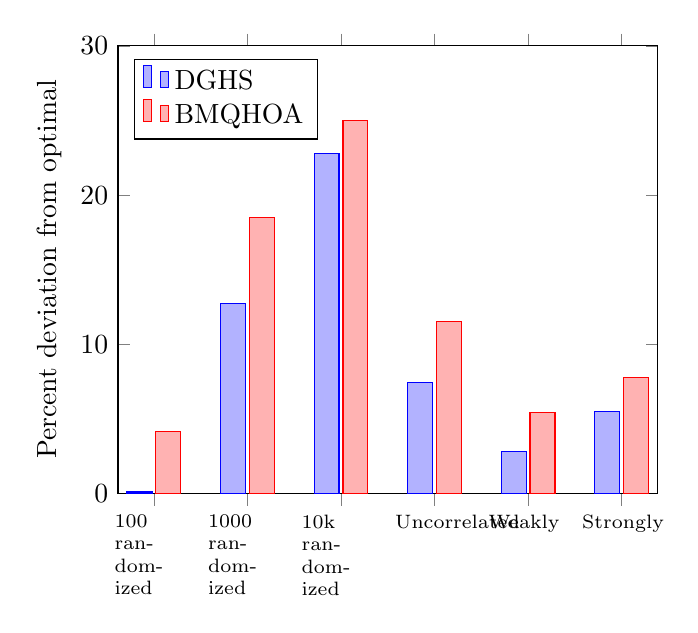
\begin{tikzpicture}
        \begin{axis} [
            ybar = .05cm,
            bar width = 9pt,
            symbolic x coords={100 randomized, 1000 randomized, 10k randomized, Uncorrelated, Weakly, Strongly},
            x tick label style={font=\scriptsize,text width=1cm,align=left},
            ymin=0,
            ylabel = Percent deviation from optimal, 
            legend cell align={left},
            legend pos = north west,
            %ytick = data,+
            enlarge y limits = {value = .2, upper},
            enlarge x limits = {abs = 13pt}
        ]
        \addplot+[] coordinates {
            (100 randomized, 0.12)
            (1000 randomized, 12.73)
            (10k randomized, 22.78)
            (Uncorrelated, 7.44)
            (Weakly, 2.81)
            (Strongly, 5.52)
        };
        \addplot+[] coordinates {
            (100 randomized, 4.17)
            (1000 randomized, 18.50)
            (10k randomized, 25.02)
            (Uncorrelated, 11.56)
            (Weakly, 5.42)
            (Strongly, 7.77)
        };
        
        \legend {DGHS, BMQHOA};
        \end{axis}
    \end{tikzpicture}
    \caption{Mean percentage deviation from optimal across all datasets} \label{deviation-graph}
    %\vfill
    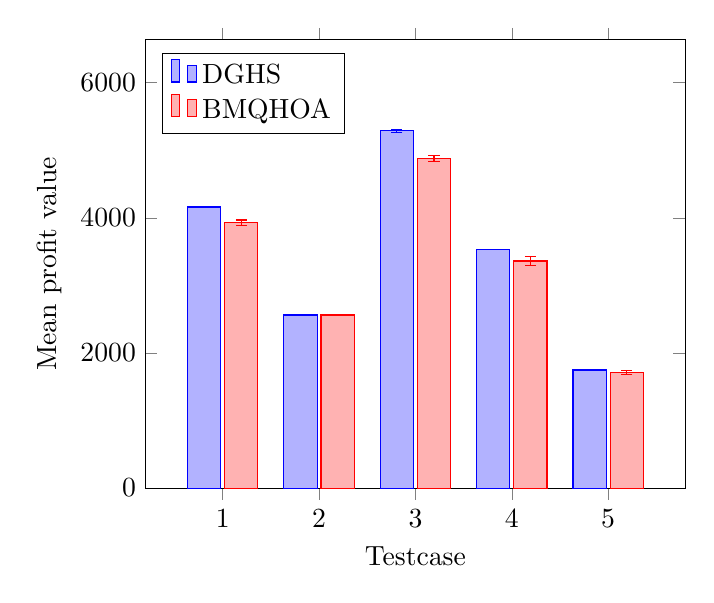
\begin{tikzpicture}
        \begin{axis} [
            ybar = .05cm,
            bar width = 12pt,
            xmin = 1,
            xmax = 5,
            ymin=0,
            xlabel = Testcase,
            ylabel = Mean profit value,
            legend cell align={left},
            legend pos = north west,
            %ytick = data,
            y tick label style={
            /pgf/number format/1000 sep=},
            enlarge y limits = {value = .25, upper},
            enlarge x limits = {abs = .8}
        ]
        \addplot+ [
                error bars/.cd,
                    y dir=both,
                    % (changed from `y explicit` so the error bars are (clearly) visible
                    y explicit ,
            ] coordinates {
                (1, 4160.33) +- (0,3.5)
                (2, 2561) +- (0,0)
                (3, 5288) +- (0,19.667)
                (4,3535) +- (0,0)
                (5,1747) +- (0,0)
            };
        \addplot+ [
                error bars/.cd,
                    y dir=both,
                    % (changed from `y explicit` so the error bars are (clearly) visible
                    y explicit ,
            ] coordinates {
                (1, 3926.83) +- (0,40.27613023)
                (2, 2561) +- (0,0)
                (3, 4879) +- (0,46.18224767)
                (4,3360.66) +- (0,68.9627919)
                (5,1711.5) +- (0,25.71186497)
            };
        \legend {DGHS, BMQHOA};
        \end{axis}
    \end{tikzpicture}
    \caption{Mean of profit values for 100 randomized items} \label{100-graph}
\end{figure}

%1000+10k random items mean and stdev graph
\begin{figure}[hbt!]
\centering
    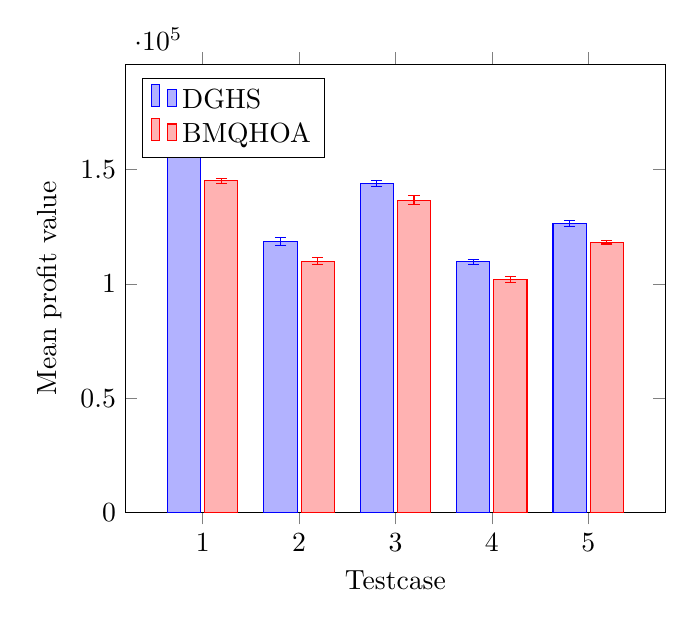
\begin{tikzpicture}
        \begin{axis} [
            ybar = .05cm,
            bar width = 12pt,
            xmin = 1,
            xmax = 5,
            ymin = 0,
            xlabel = Testcase,
            ylabel = Mean profit value,
            legend cell align={left},
            legend pos = north west,
            %ytick = data,
            y tick label style={
            /pgf/number format/1000 sep=},
            enlarge y limits = {value = .25, upper},
            enlarge x limits = {abs = .8}
        ]
        \addplot+ [
                error bars/.cd,
                    y dir=both,
                    % (changed from `y explicit` so the error bars are (clearly) visible
                    y explicit ,
            ] coordinates {
                (1, 156083.83) +- (0,830.04)
                (2, 118603.83) +- (0,1904.70)
                (3, 144070.00) +- (0,1343.77)
                (4, 109734.33) +- (0,1037.03)
                (5, 126366.17) +- (0,1236.73)
            };
        \addplot+ [
                error bars/.cd,
                    y dir=both,
                    % (changed from `y explicit` so the error bars are (clearly) visible
                    y explicit ,
            ] coordinates {
                (1, 145086.50) +- (0,1035.46)
                (2, 109876.33) +- (0,1540.63)
                (3, 136622.67) +- (0,2042.95)
                (4,101951.33) +- (0,1271.88)
                (5,118291.17) +- (0,799.79)
            };
        \legend {DGHS, BMQHOA};
        \end{axis}
    \end{tikzpicture}
\caption{Mean of profit values for 1000 randomized items} \label{1000-graph}
%\end{figure}

%10k random items mean and stdev graph
%\begin{figure}[hbt!]
%\centering
    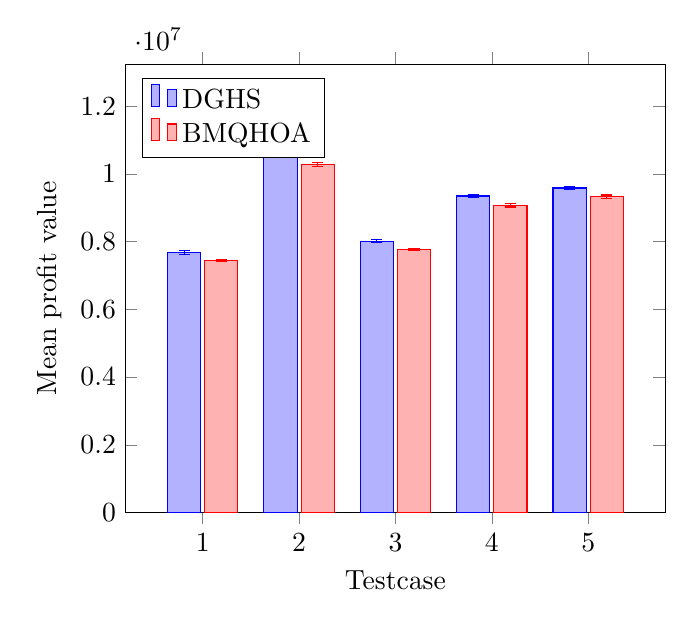
\begin{tikzpicture}
        \begin{axis} [
            ybar = .05cm,
            bar width = 12pt,
            xmin = 1,
            xmax = 5,
            ymin = 0,
            xlabel = Testcase,
            ylabel = Mean profit value,
            %ytick = data,
            legend cell align={left},
            legend pos = north west,
            y tick label style={
            /pgf/number format/1000 sep=},
            enlarge y limits = {value = .25, upper},
            enlarge x limits = {abs = .8}
        ]
        \addplot+ [
                error bars/.cd,
                    y dir=both,
                    % (changed from `y explicit` so the error bars are (clearly) visible
                    y explicit ,
            ] coordinates {
                (1, 7681910.333) +- (0, 51555.40)
                (2, 10567302) +- (0, 23956.32)
                (3, 8014906) +- (0, 39449.15)
                (4, 9347061.67) +- (0, 56967.67)
                (5, 9583139.17) +- (0, 55816.61)
            };
        \addplot+ [
                error bars/.cd,
                    y dir=both,
                    % (changed from `y explicit` so the error bars are (clearly) visible
                    y explicit ,
            ] coordinates {
                (1, 7438487.17) +- (0, 29887.18)
                (2, 10276681.83) +- (0, 50507.36)
                (3, 7774520.83) +- (0, 34559.11)
                (4, 9075476.00) +- (0, 53168.02)
                (5, 9330322.17) +- (0, 46301.35)
            };
        \legend {DGHS, BMQHOA};
        \end{axis}
    \end{tikzpicture}
\caption{Mean of profit values for 10k randomized items} \label{10k-graph}
\end{figure}

%all correlations of items mean and stdev graph
\begin{figure}[hbt!]
    \centering
    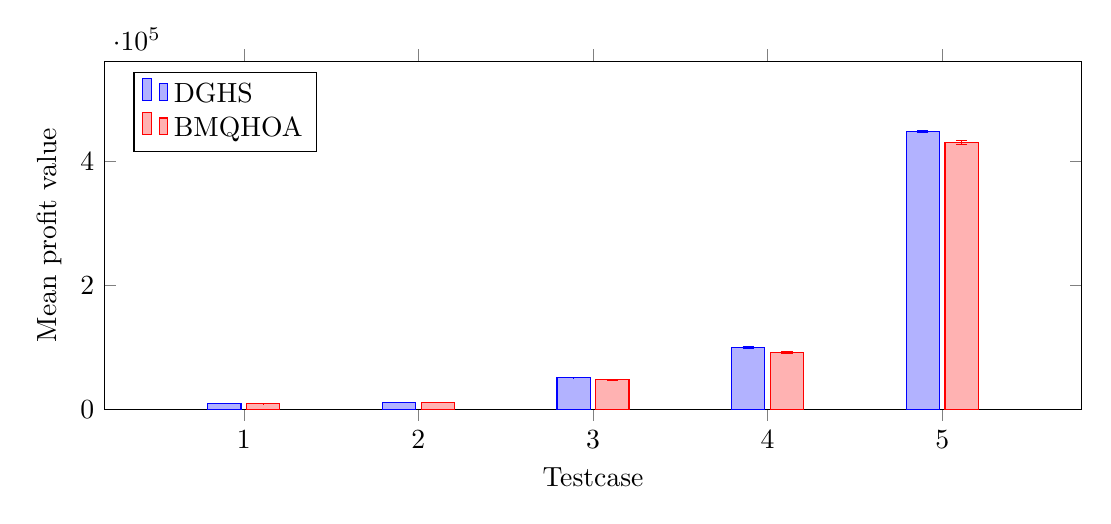
\begin{tikzpicture}
        \begin{axis} [
            ybar,
            bar width = 12pt,
            width = 14cm,
            height = 6cm,
            xlabel = Testcase,
            ylabel = Mean profit value,
            xmin = 1,
            xmax = 5,
            ymin = 0,
            legend cell align={left},
            legend pos = north west,
            %x tick label style={rotate=45},
            xtick = data,
            ymin=0,
            %ytick = data,
            y tick label style={/pgf/number format/1000 sep=},
            enlarge y limits = {value = .25, upper},
            enlarge x limits = {abs = .8}
            %enlarge x limits = {abs = .8}
        ]
        \addplot+ [
                error bars/.cd,
                    y dir=both,
                    % (changed from `y explicit` so the error bars are (clearly) visible
                    y explicit ,
            ] coordinates {
                (1, 9147) +- (0, 0.00)
                (2, 11238.00) +- (0, 0.00)
                (3, 51019.50) +- (0, 437.85)
                (4, 99036.17) +- (0, 1544.34)
                (5, 448975.00) +- (0, 1135.46)
            };
        \addplot+ [
                error bars/.cd,
                    y dir=both,
                    % (changed from `y explicit` so the error bars are (clearly) visible
                    y explicit ,
            ] coordinates {
                (1, 8974.50) +- (0, 147.24)
                (2, 10976.50) +- (0, 154.37)
                (3, 47401.50) +- (0, 841.76)
                (4, 91725.83) +- (0, 1346.24)
                (5, 431259.67) +- (0, 3049.43)
            };
        \legend {DGHS, BMQHOA};
        \end{axis}
    \end{tikzpicture}
\caption{Mean of profit values for uncorrelated items} \label{uncorrelated-graph}
%\end{figure}

%\begin{figure}[hbt!]
    %\centering
    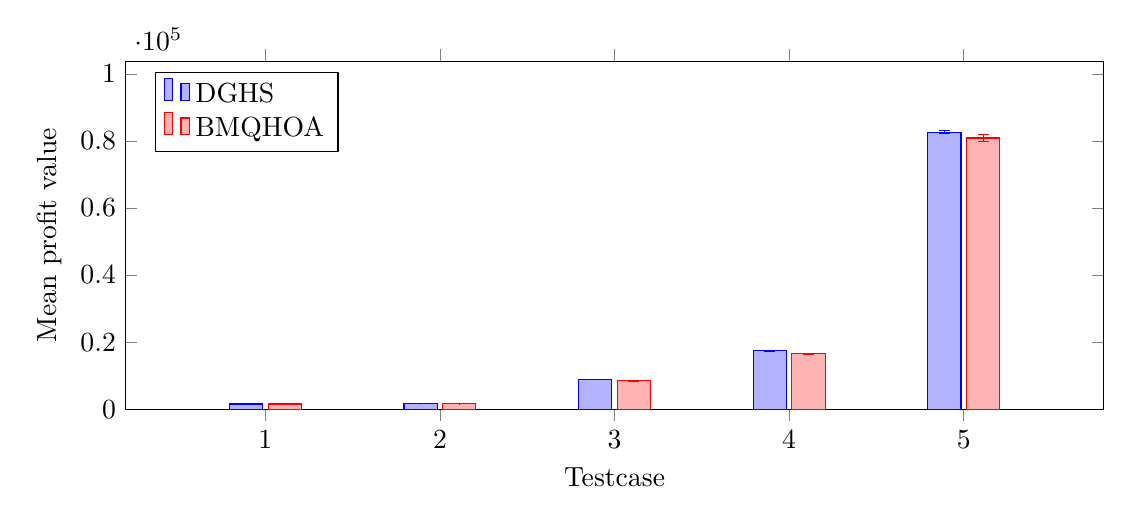
\begin{tikzpicture}
        \begin{axis} [
            ybar,
            bar width = 12pt,
            width = 14cm,
            height = 6cm,
            xlabel = Testcase,
            ylabel = Mean profit value,
            xmin = 1,
            xmax = 5,
            ymin=0,
            legend cell align={left},
            legend pos = north west,
            %x tick label style={rotate=45},
            xtick = data,
            %ytick = data,
            y tick label style={/pgf/number format/1000 sep=},
            enlarge y limits = {value = .25, upper},
            enlarge x limits = {abs = .8}
            %enlarge x limits = {abs = .8}
        ]
        \addplot+ [
                error bars/.cd,
                    y dir=both,
                    % (changed from `y explicit` so the error bars are (clearly) visible
                    y explicit ,
            ] coordinates {
                (1, 1514) +- (0, 0.00)
                (2, 1627.666667) +- (0, 2.422120283)
                (3, 8907.333333) +- (0, 27.56567914)
                (4, 17371.83333) +- (0, 126.7665834)
                (5, 82681.33333) +- (0, 390.9842282)
            };
        \addplot+ [
                error bars/.cd,
                    y dir=both,
                    % (changed from `y explicit` so the error bars are (clearly) visible
                    y explicit ,
            ] coordinates {
                (1, 1508.166667) +- (0, 6.823977335)
                (2, 1613.666667) +- (0, 16.74116683)
                (3, 8435.333333) +- (0, 60.6025302)
                (4, 16539) +- (0, 133.9596954)
                (5, 80900.66667) +- (0, 970.7196643)
            };
        \legend {DGHS, BMQHOA};
        \end{axis}
    \end{tikzpicture}
\caption{Mean of profit values for weakly correlated items} \label{weakly-graph}
%\end{figure}

%\begin{figure}[hbt!]
    %\centering
    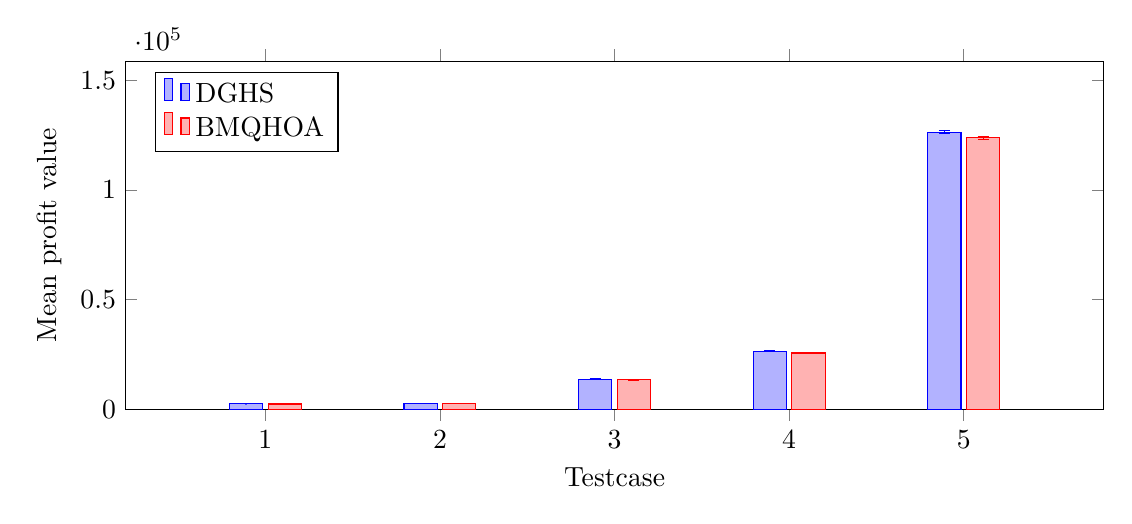
\begin{tikzpicture}
        \begin{axis} [
            ybar,
            bar width = 12pt,
            xlabel = Testcase,
            ylabel = Mean profit value,
            width = 14cm,
            height = 6cm,
            xmin = 1,
            xmax = 5,
            ymin = 0,
            legend cell align={left},
            legend pos = north west,
            %x tick label style={rotate=45},
            xtick = data,
            %ytick = data,
            y tick label style={/pgf/number format/1000 sep=},
            enlarge y limits = {value = .25, upper},
            enlarge x limits = {abs = .8}
            %enlarge x limits = {abs = .8}
        ]
        \addplot+ [
                error bars/.cd,
                    y dir=both,
                    % (changed from `y explicit` so the error bars are (clearly) visible
                    y explicit ,
            ] coordinates {
                (1, 2391.666667) +- (0, 6.08824003)
                (2, 2697) +- (0, 0)
                (3, 13682.5) +- (0, 60.05580738)
                (4, 26444.66667) +- (0, 240.8407496)
                (5, 126448) +- (0, 615.61384)
            };
        \addplot+ [
                error bars/.cd,
                    y dir=both,
                    % (changed from `y explicit` so the error bars are (clearly) visible
                    y explicit ,
            ] coordinates {
                (1, 2327.333333) +- (0, 48.55375028)
                (2, 2658.666667) +- (0, 48.81666382)
                (3, 13334.66667) +- (0, 182.9160099)
                (4, 25604) +- (0, 91.32579044)
                (5, 123813.8333) +- (0, 773.1955553)
            };
        \legend {DGHS, BMQHOA};
        \end{axis}
    \end{tikzpicture}
\caption{Mean of profit values for strongly correlated items} \label{strongly-graph}
\end{figure}

\clearpage

\newpage 

\section{Not finished - Discussion}
As one can see in Figure 1, the DGHS algorithm deviates more than the BMQHOA algorithm in all datasets. One can draw the conclusion that the DGHS algorithm is superior.

In Table 7 and the corresponding Figure 1, the data shows that testcases with a greater number of items have resulted in greater deviations from the optimal. Both algorithms are probabilistic and work by generating new candidate solutions, and replacing worse solutions with better ones. As the generation process is only run 100 times in both algorithms, and as there are $2^{noItems}$ different possible solutions (possibly violating the constraints), the likelihood of finding optimal or near-optimal solutions decreases.

The BMQHOA algorithm only flips 1 item toward the corresponding item in the current best solution during the solution generation process. The DGHS harmony generation, on the other hand, probabilistically considers every item for flipping toward the best solution, depending on the current iteration's HMCR value.  As the BMQHOA has produced worse profit values, it can be suggests that a greater level of evolution toward current best solutions is advantageous. 

\newpage

\bibliographystyle{unsrt}
\bibliography{references}


\section{Appendix}
\begin{table}[!h]\centering
    \caption{Randomized 100 items} \label{random100}
    \begin{tabu}{|c|c|c|c|c|c|c|}
        \tabucline[1pt]{1-6} 
        Testcase & 1 & 2 & 3 & 4 & 5 \\ [-1pt] \tabucline[1pt]{1-6} 
        Optimal & 4169 & 2561 & 5309 & 3535 & 1747 \\ [-1pt] \tabucline[1pt]{1-6} 
        \multirow{6}{*}{DGHS} & 4163 & 2561 & 5254 & 3535 & 1747 \\ \cline{2-6}
        & 4163 & 2561 &5292 &3535 &1747 \\ \cline{2-6} 
        &4161 &2561 &5307 &3535 &1747 \\ \cline{2-6} 
        &4163 &2561 &5282 &3535 &1747 \\ \cline{2-6} 
        &4155 &2561 &5307 &3535 &1747 \\ \cline{2-6} 
        &4157 &2561 &5286 &3535 &1747 \\[-1pt] \tabucline[1pt]{1-6}
        \multirow{6}{*}{BMQHOA} &3895 &2561 &4952 &3398 &1734 \\\cline{2-6} 
        &3939 &2561 &4871 &3380 &1728 \\\cline{2-6} 
        &3870 &2561 &4890 &3298 &1705 \\\cline{2-6} 
        &3948 &2561 &4829 &3435 &1718 \\\cline{2-6} 
        &3984 &2561 &4832 &3255 &1663 \\\cline{2-6} 
        &3925 &2561 &4900 &3398 &1721 \\[-1pt] \tabucline[1pt]{1-6}
    \end{tabu}
\end{table}

\begin{table}[!h] \centering
    \caption{Randomized 1000 items} \label{random1000}
    \begin{tabu}{|c|[1pt]c|c|c|c|c|c|}
        \tabucline[1pt]{1-6} 
        Testcase & 1 & 2 & 3 & 4 & 5 \\ [-1pt] \tabucline[1pt]{1-6} 
        Optimal & 4169 & 2561 & 5309 & 3535 & 1747 \\ [-1pt] \tabucline[1pt]{1-6} 
        \multirow{6}{*}{DGHS} & 156898 & 119888 & 141878 & 110608 & 128009 \\ \cline{2-6}
        &155104 &117086 &143322 &108732 &124714 \\ \cline{2-6} 
        &155849 &117110 &145381 &108973 &125400 \\ \cline{2-6} 
        &155171 &116958 &145411 &109414 &126089 \\ \cline{2-6} 
        &156929 &118957 &143984 &109292 &126532 \\ \cline{2-6} 
        &156552 &121624 &144444 &111387 &127453 \\ [-1pt] \tabucline[1pt]{1-6}
        \multirow{6}{*}{BMQHOA} &146187 &110066 &136620 &103073 &117832 \\ \cline{2-6} 
        &146215 &107880 &133731 &101385 &117207 \\ \cline{2-6} 
        &145231 &109374 &134981 &99977 &119272 \\ \cline{2-6} 
        &143511 &108754 &137715 &102749 &117836 \\ \cline{2-6} 
        &144522 &112065 &137185 &101318 &118550 \\ \cline{2-6} 
        &144853 &111119 &139504 &103206 &119050 \\ [-1pt] \tabucline[1pt]{1-6}
    \end{tabu}
\end{table}

\begin{table}[!h] \centering
    \caption{Randomized 10k items} \label{random10k}
    \begin{tabu}{|c|[1pt]c|c|c|c|c|c|}
        \tabucline[1pt]{1-6} 
        Testcase & 1 & 2 & 3 & 4 & 5 \\ [-1pt] \tabucline[1pt]{1-6} 
        Optimal &9927473 &13743791 &10286004 &12155538 &12446154 \\ [-1pt] \tabucline[1pt]{1-6} 
        \multirow{6}{*}{DGHS} &7667918 &10556718 &8064941 &9425334 &9545542 \\ \cline{2-6}
        &7738704 &10587645 &8059383 &9305736 &9547723 \\ \cline{2-6} 
        &7590747 &10523899 &7986766 &9304266 &9679149 \\ \cline{2-6} 
        &7680907 &10571613 &8018689 &9377397 &9621182 \\ \cline{2-6} 
        &7719598 &10584319 &7983856 &9386494 &9538807 \\ \cline{2-6} 
        &7693588 &10579618 &7975801 &9283143 &9566432 \\ [-1pt] \tabucline[1pt]{1-6}
        \multirow{6}{*}{BMQHOA} &7483414 &10312486 &7823273 &9090434 &9368506 \\ \cline{2-6} 
        &7398497 &10196292 &7796298 &9030552 &9332763 \\ \cline{2-6} 
        &7429280 &10328466 &7768443 &9107012 &9246868 \\ \cline{2-6} 
        &7452071 &10285331 &7786678 &9064793 &9351821 \\ \cline{2-6} 
        &7450200 &10236135 &7737071 &9006745 &9312696 \\ \cline{2-6} 
        &7417461 &10301381 &7735362 &9153320 &9369279 \\ [-1pt] \tabucline[1pt]{1-6}
    \end{tabu}
\end{table}

\begin{table}[!h] \centering
    \caption{Uncorrelated Dataset} \label{uncorrelated}
    \begin{tabu}{|c|[1pt]c|c|c|c|c|c|}
        \tabucline[1pt]{1-6} 
        Testcase & 1 & 2 & 3 & 4 & 5 \\ [-1pt] \tabucline[1pt]{1-6} 
        Optimal &9147 &11238 &54503 &110625 &563647 \\ [-1pt] \tabucline[1pt]{1-6} 
        \multirow{6}{*}{DGHS} &9147 &11238 &51166 &100770 &450386 \\ \cline{2-6}
        &9147 &11238 &50911 &98217 &448025 \\ \cline{2-6} 
        &9147 &11238 &50674 &100153 &449887 \\ \cline{2-6} 
        &9147 &11238 &51168 &100285 &447368 \\ \cline{2-6} 
        &9147 &11238 &51720 &97570 &448856 \\ \cline{2-6} 
        &9147 &11238 &50478 &97222 &449328 \\ [-1pt] \tabucline[1pt]{1-6}
        \multirow{6}{*}{BMQHOA} &8990 &11005 &47569 &91878 &429245 \\ \cline{2-6} 
        &9147 &11031 &47106 &90966 &437054 \\ \cline{2-6} 
        &8911 &10759 &47773 &93434 &432253 \\ \cline{2-6} 
        &9147 &11168 &47302 &91491 &429942 \\ \cline{2-6} 
        &8810 &10826 &48608 &89694 &429823 \\ \cline{2-6} 
        &8842 &11070 &46051 &92892 &429241 \\ [-1pt] \tabucline[1pt]{1-6}
    \end{tabu}
\end{table}

\begin{table}[!h] \centering
    \caption{Weakly Correlated Dataset} \label{weakly-correlated}
    \begin{tabu}{|c|[1pt]c|c|c|c|c|c|}
        \tabucline[1pt]{1-6} 
        Testcase & 1 & 2 & 3 & 4 & 5 \\ [-1pt] \tabucline[1pt]{1-6} 
        Optimal &1514 &1634 &9052 &18051 &90204 \\ [-1pt] \tabucline[1pt]{1-6} 
        \multirow{6}{*}{DGHS} &1514 &1627 &8917 &17251 &82712 \\ \cline{2-6}
        &1514 &1629 &8898 &17224 &82571 \\ \cline{2-6} 
        &1514 &1629 &8899 &17409 &82348 \\ \cline{2-6} 
        &1514 &1629 &8892 &17519 &83330 \\ \cline{2-6} 
        &1514 &1623 &8880 &17321 &82254 \\ \cline{2-6} 
        &1514 &1629 &8958 &17507 &82873 \\ [-1pt] \tabucline[1pt]{1-6}
        \multirow{6}{*}{BMQHOA} &1512 &1633 &8516 &16578 &80645 \\ \cline{2-6} 
        &1512 &1625 &8493 &16493 &80431 \\ \cline{2-6} 
        &1514 &1604 &8412 &16415 &80591 \\ \cline{2-6} 
        &1501 &1626 &8385 &16495 &80443 \\ \cline{2-6} 
        &1498 &1604 &8362 &16463 &82873 \\ \cline{2-6} 
        &1512 &1590 &8444 &16790 &80421 \\ [-1pt] \tabucline[1pt]{1-6}
    \end{tabu}
\end{table}

\begin{table}[!h] \centering
    \caption{Strongly correlated Dataset} \label{strongly-correlated}
    \begin{tabu}{|c|[1pt]c|c|c|c|c|c|}
        \tabucline[1pt]{1-6} 
        Testcase & 1 & 2 & 3 & 4 & 5 \\ [-1pt] \tabucline[1pt]{1-6} 
        Optimal &2397 &2697 &14390 &28919 &146919 \\ [-1pt] \tabucline[1pt]{1-6} 
        \multirow{6}{*}{DGHS} &2390 &2697 &13586 &26711 &126318 \\ \cline{2-6}
        &2390 &2697 &13690 &26708 &127616 \\ \cline{2-6} 
        &2397 &2697 &13673 &26311 &126212 \\ \cline{2-6} 
        &2381 &2697 &13686 &26513 &126513 \\ \cline{2-6} 
        &2396 &2697 &13685 &26114 &126212 \\ \cline{2-6} 
        &2396 &2697 &13775 &26311 &125817 \\ [-1pt] \tabucline[1pt]{1-6}
        \multirow{6}{*}{BMQHOA} &2294 &2596 &13183 &25712 &124918 \\ \cline{2-6} 
        &2296 &2681 &13090 &25583 &123503 \\ \cline{2-6} 
        &2390 &2696 &13570 &25706 &123613 \\ \cline{2-6} 
        &2297 &2689 &13490 &25498 &123217 \\ \cline{2-6} 
        &2390 &2596 &13288 &25515 &123017 \\ \cline{2-6} 
        &2297 &2694 &13387 &25610 &124615 \\ [-1pt] \tabucline[1pt]{1-6}
    \end{tabu}
\end{table}



\end{document}
